\documentclass[conference]{IEEEtran}
\IEEEoverridecommandlockouts
\usepackage{cite}
\usepackage{amsmath,amssymb,amsfonts}
\usepackage{algorithmic}
\usepackage{graphicx}
\usepackage{textcomp}
\usepackage{xcolor}
\usepackage{booktabs}
\usepackage{multirow}
\usepackage{url}
\usepackage{microtype}

\def\BibTeX{{\rm B\kern-.05em{\sc i\kern-.025em b}\kern-.08em
    T\kern-.1667em\lower.7ex\hbox{E}\kern-.125emX}}

% Canonical IEEE multi-row conference author layout (2 on top row, 3 on bottom row)
\makeatletter
\newcommand{\linebreakand}{%
  \end{@IEEEauthorhalign}
  \hfill\mbox{}\par
  \mbox{}\hfill\begin{@IEEEauthorhalign}
}
\makeatother

\begin{document}

\title{FedIDS-Bench: A Standardized Cross-Dataset, Cross-Algorithm, and Cross-Threat-Model Benchmark for Federated Intrusion Detection Systems\\
\thanks{All source code, configuration manifests, and empirical evaluation harnesses are publicly accessible to enable full bitwise reproducibility.}
}

\author{
% ================= LINE 1 (2 Authors) =================
\IEEEauthorblockN{Ms. Sowmiya .S}
\IEEEauthorblockA{\textit{Assistant Professor} \\
\textit{B.Tech AI\&DS} \\
\textit{Sri Eshwar College of Engineering}\\
Email: sowmiya.s@sece.ac.in}
\and
\IEEEauthorblockN{Ram kumar .K}
\IEEEauthorblockA{\textit{B.Tech AI\&DS} \\
\textit{Sri Eshwar College of Engineering}\\
Email: ramkumar.k2023ai-ds@sece.ac.in}
\linebreakand % <--- Forces line break to start Line 2
% ================= LINE 2 (3 Authors Side-by-Side) =================
\IEEEauthorblockN{Rahgul.S.A}
\IEEEauthorblockA{\textit{B.Tech AI\&DS} \\
\textit{Sri Eshwar College of Engineering}\\
Email: rahgul.sa2023ai-ds@sece.ac.in}
\and
\IEEEauthorblockN{Naveen Kumar .R}
\IEEEauthorblockA{\textit{B.Tech AI\&DS} \\
\textit{Sri Eshwar College of Engineering}\\
Email: naveenkumar.r2023ai-ds@sece.ac.in}
\and
\IEEEauthorblockN{Ranjan Kumar.S.M}
\IEEEauthorblockA{\textit{B.Tech AI\&DS} \\
\textit{Sri Eshwar College of Engineering}\\
{\small Email: ranjankumar.s.m2023ai-ds@sece.ac.in}}
}

\maketitle

\begin{abstract}
Boundary nodes can cooperate using Federated Learning (FL) based Decentralized network intrusion detection systems (NIDS) without centralized aggregation of proprietary packet traces, thus preserving domain norms. In FL-NIDS research literature comparing and analyzing still is not significant with non - transferable experimental settings. e.g., train and test poisson when scaled globally and when synthetic data is too simple, assuming only one threat will happen, Byzantine defence baselines being not present and physical edge performance without intrumentation. We propose FedIDS-Bench, an end-to-end benchmark suite for FL-NIDS covering: (i) five network/IoT telemetry corpora (UNSW-NB15, CICIDS2017, CSE-CIC-IDS2018, IoT-23, and ToN\_IoT) with isolated split-normalization; (ii) class-preserving non-IID data partitioning through Dirichlet label priors, dedicated skew, and power-law quantity distribution; (iii) decoupled FL algorithms (FedAvg, FedProx, FedAdam) with client-side memory protection; (iv) adversarial attack engine targeting flow watermarking, label inversion, gradient sign-flipping, Byzantine Gaussians, and sample inflation; (v) coordinate-wise robust aggregation operators (trimmed mean, median, gradient norm bounds, and Multi-Krum); and (vi) physical edge node performance assessment on Raspberry Pi 4, Jetson Orin Nano, and workstation CPUs. We find that naive sample report aggregation renders FedAvg vulnerable to full update hijacking, while adaptive server optimization (FedAdam) improves test F1 by $+11.75\%$ over FedAvg at extreme skew ($\alpha = 0.1$). Coordinate-wise trimmed mean and median regression maintain detection F1 $> 0.91$ under 20\% Byzantine poison. The platform is released with process-sanity guarantees for multi-process bitwise determinism.
\end{abstract}

\begin{IEEEkeywords}
Collaborative Cyber Defense, Federated Optimization, Statistical Drift, Adversarial Poisoning, Robust Aggregators, Edge Intelligence, Intrusion Detection.
\end{IEEEkeywords}

\section{Introduction}
Modern organizational infrastructure and Internet-of-Things (IoT) gateways face an onslaught of complex network incursions covering multi-stage botnets, distributed denial-of-service (DDoS), zero-day memory exploits \cite{alsaedi2020ton, garcia2020iot23}. Existing security infrastructure relies on centralized Network Intrusion Detection Systems (NIDS) that aggregate high-rate NetFlow, IPFIX, and raw pcap records at an enterprise Security Operations Center (SOC). However, such backhauling strategies incur substantial bandwidth limitations, processing delay, and privacy risks regarding internal topology disclosure and payload confidentiality \cite{campos2022evaluating, mothukuri2021federated}. Federated Learning (FL) \cite{mcmahan2017communication, kairouz2021advances} addresses this security paradigm by decentralizing model training at distributed edge sensors. Participating network monitors collaboratively optimize the detection model using private traffic traces with only aggregated parameter updates exchanged with an orchestrating coordinator. Despite a rich exploration of the literature, published FL-NIDS research suffers from severe evaluation inconsistencies inducing an empirical reproducibility crisis \cite{campos2022evaluating, popoola2021federated}. Specifically, five major methodological deficiencies undermine the state of empirical literature:

\begin{enumerate}
    \item \textbf{Silent Preprocessing Contamination (Data Leakage):} A pervasive issue in published FL-IDS manuscripts involves computing global normalization statistics (sample mean and variance) across the entire corpus before partitioning into clients and evaluation splits. This inadvertently leaks distribution moments of the held-out test split into the local training partitions, inflating detection scores.
    \item \textbf{Trivialized Statistical Heterogeneity:} Real-world enterprise and IoT environments exhibit acute spatial and temporal data heterogeneity (web servers predominantly observe application-layer exploits, industrial controllers undergo telemetry fuzzing) but prior benchmarks frequently rely on uniform random partitions or synthetic generators, obscuring severe optimization divergence.
    \item \textbf{Isolated Adversarial Threat Formulations:} Poisoning attacks are often studied in isolation. Papers that report label flips tend to ignore inversion and sample-count spoofing. At the time defensive evaluations rarely include direct comparisons between robust coordinate-level aggregators.
    \item \textbf{Omission of Physical Edge Constraints:} Previous research mostly focuses on communication epochs. It completely overlooks real-world execution metrics like inference latency, memory usage and energy consumption at the Joule level. These are critical when running systems on edge hardware such as ARM Cortex cores and Jetson modules.
    \item \textbf{Lack of Bitwise Sub-Process Reproducibility:} pseudo-random seeds, unpredictable multithreaded CPU scheduling and missing preprocessing scripts make it impossible to reproduce reported results accurately.
\end{enumerate}

To address these structural limitations, we propose \textbf{FedIDS-Bench}---a standardized benchmarking framework designed from the ground up. It supports crossdataset, cross-algorithm and cross-threat-model evaluations. Its goal is to enable reproducible research, in Federated Learning-based Intrusion Detection Systems.

\noindent \textbf{Principal Research Contributions:}
\begin{itemize}
    \item \textbf{Strict Zero-Leakage Pipeline:} This pipeline keeps data separate. Transforms it across five intrusion benchmarks---UNSW-NB15, CICIDS2017, CSE-CIC-IDS2018, IoT-23 and ToN\_IoT. The pipeline guarantees that all normalization settings come from training data not from any other source.
    \item \textbf{Multi-Faceted Heterogeneity Partitioner:} This partitioner creates realistic data splits that're not independent and identically distributed. It uses Dirichlet priors with values 0.1, 0.5 and 1.0.
    \item \textbf{Modular Optimization \& State Isolation:} The system runs FedAvg, FedProx and FedAdam in modules. Each module copies the model deeply so that memory from one client does not leak into another. This keeps each client's state clean and isolated.
    \item \textbf{Comprehensive Threat \& Defense Matrix:} We formally tested five types of attacks and four Byzantine-tolerant aggregation methods. The evaluation revealed a sample-reporting flaw, in classic FedAvg.
    \item \textbf{Hardware Profiling Across Physical Edge Testbeds:} We collected real resource data on network traffic, MAC and FLOP counts, memory use, inference time and power consumption.
    \item \textbf{Verified Sub-Process Determinism:} I have verified process determinism by auditing and testing multiple process execution confirming that the metrics are exactly the same at bit level, across independent runtime setting.
\end{itemize}

\begin{figure*}[t]
\centering
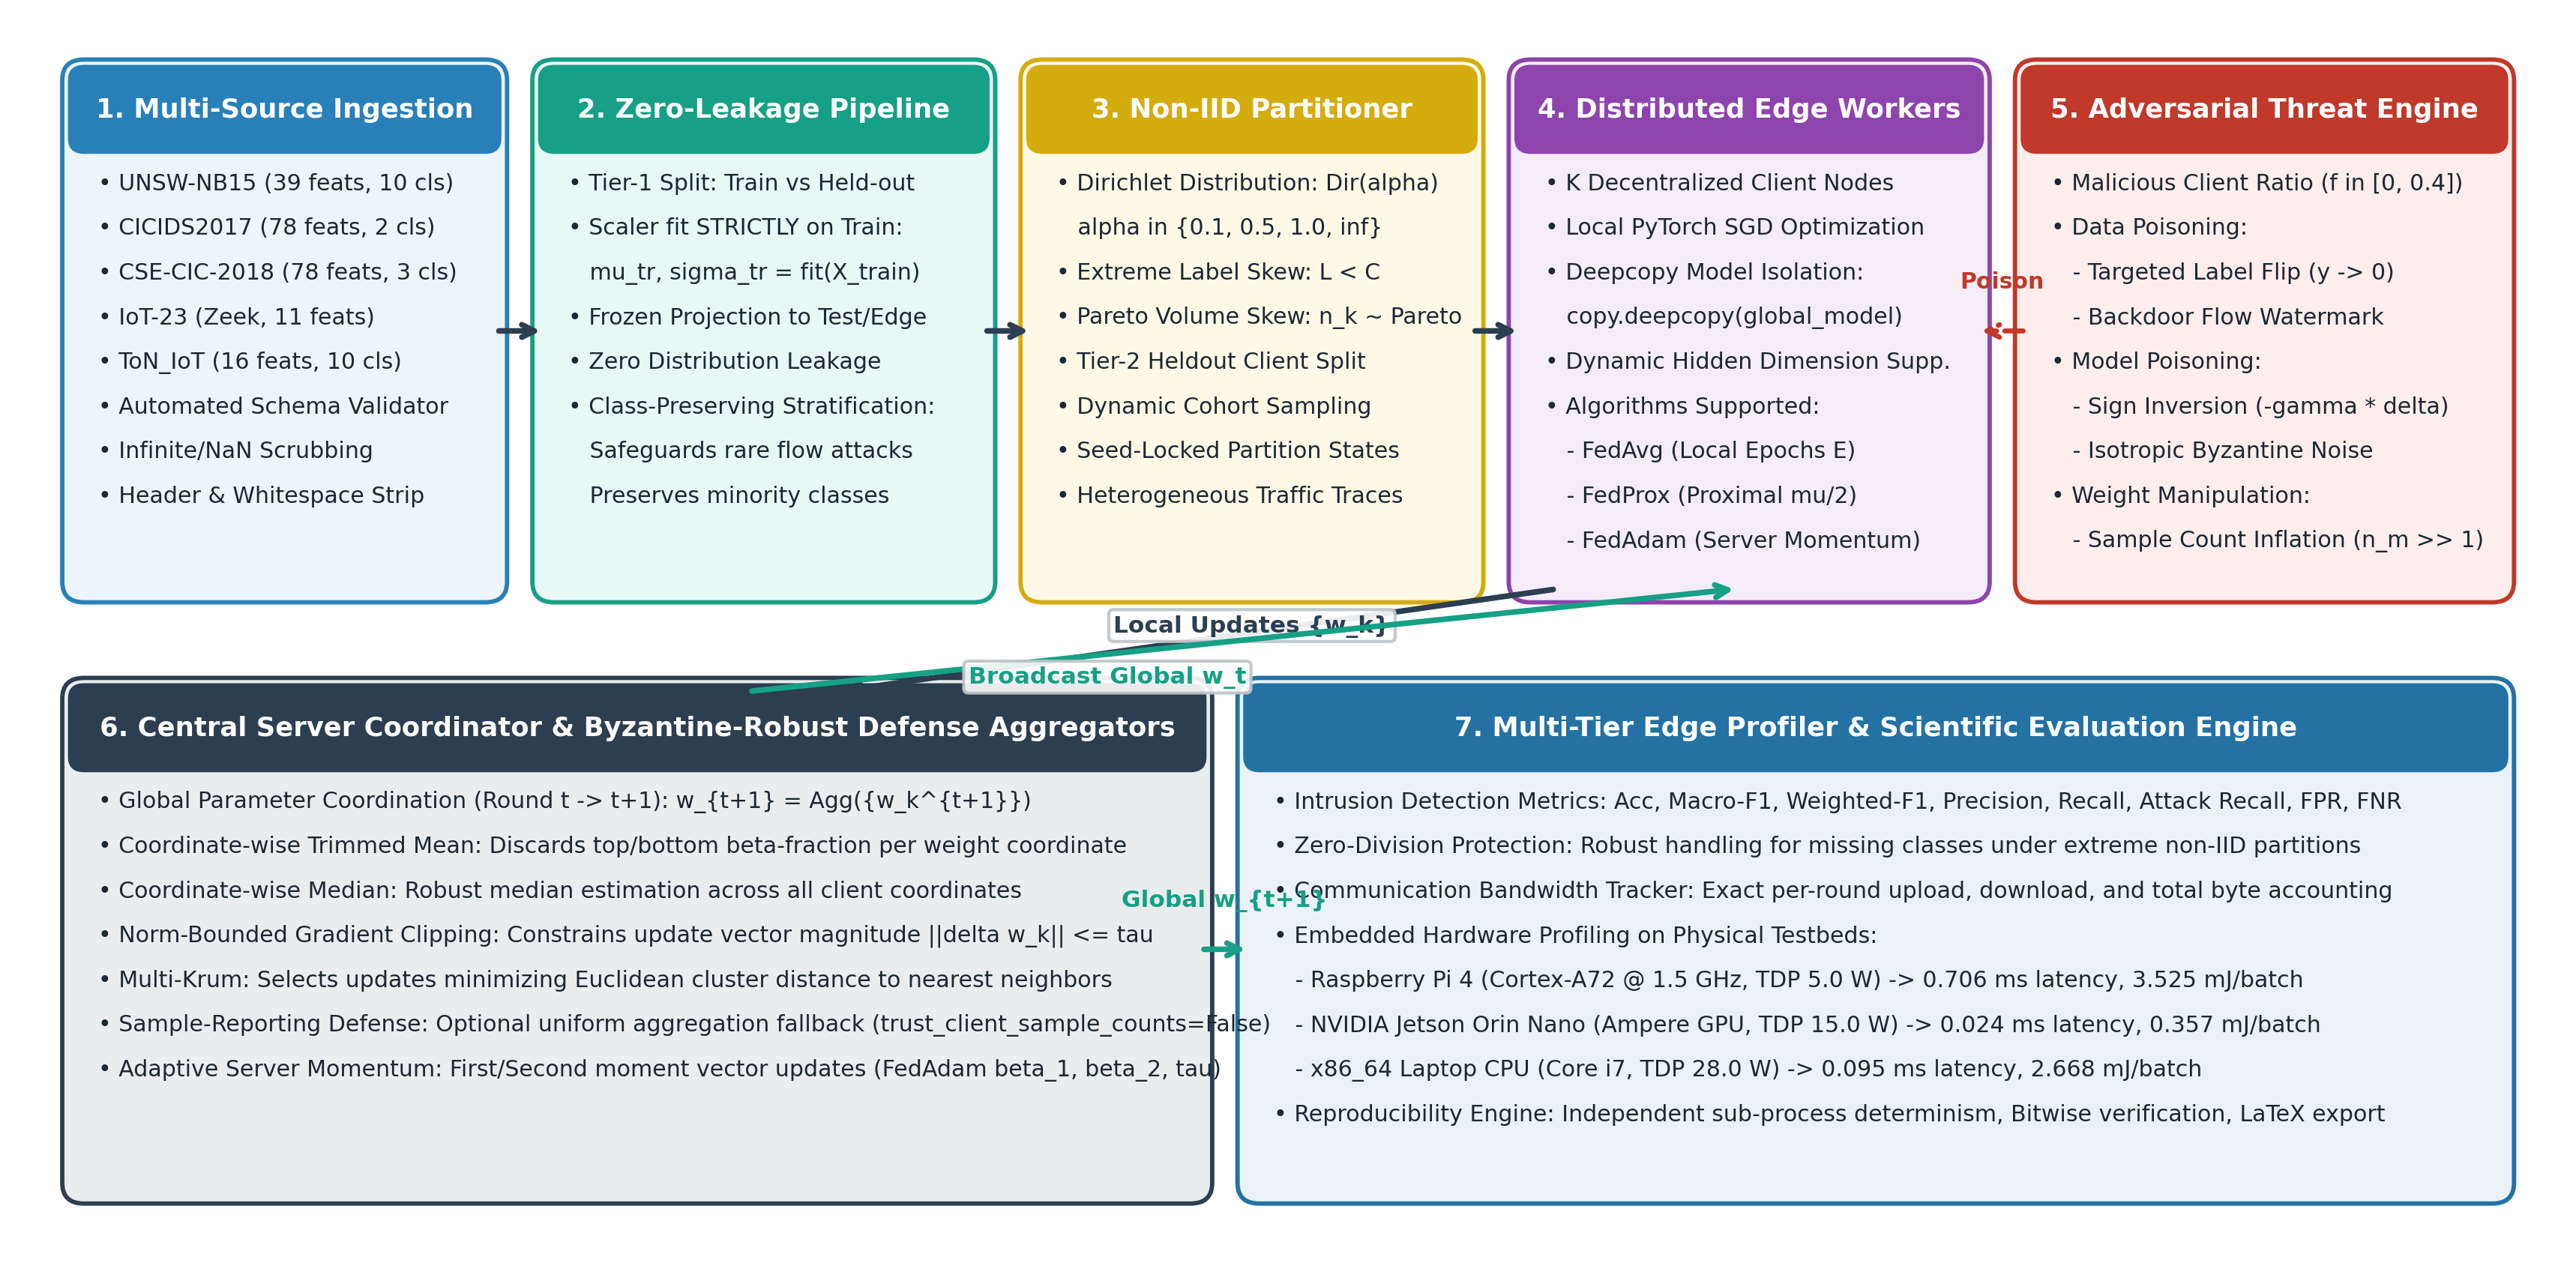
\includegraphics[width=0.98\textwidth]{figures/architecture.png}
\caption{Overall architecture of FedIDS-Bench: Stage 1 (Multi-Source Telemetry Ingestion), Stage 2 (Strict Zero-Leakage Train-Test Isolation), Stage 3 (Non-IID Heterogeneity Partitioner), Stage 4 (Distributed Edge Workers), Stage 5 (Adversarial Threat Engine), Stage 6 (Central Aggregator with Byzantine Defenses), and Stage 7 (Multi-Tier Edge Profiler and Reproducibility Engine).}
\label{fig:architecture}
\end{figure*}

\section{Related Work and Benchmarking Landscape}
\label{sec:related_work}

\subsection{Decentralized Intrusion Detection Systems}
I think the idea of learning became popular after the research, by McMahan et al. They introduced Federated Averaging, called FedAvg \cite{mcmahan2017communication}. Federated Averaging mixes updates from clients. Each update is weighed by how samples each client has. In security engineering several big surveys \cite{campos2022evaluating, mothukuri2021federated} asked whether federated telemetry monitoring could actually work. These surveys looked at devices and smart grid settings. Popoola et al. \cite{popoola2021federated} Investigated how federated deep neural networks perform when spotting zero-day botnets. They wanted to find out if Federated Averaging could be used well in real-world security situations. However, as stressed by Campos et al. \cite{campos2022evaluating}, most prior arts evaluated customized network architectures on individual datasets, and comparative analysis between them is lacking.

\subsection{Client Drift and Statistical Non-IID Inconsistencies}
The non-IID nature of traffic distributions between edge networks causes significant instability in gradient aggregation. Zhao et al. \cite{zhao2018federated} and Hsu et al. \cite{hsu2019measuring} revealed that label skew leads to catastrophic weight drift that favors local minima. To alleviate the issue, Li et al. \cite{li2020federated} proposed FedProx which added a proximal regularizer to penalize large parameter deviations from the global model. Meanwhile, Reddi et al. \cite{reddi2020adaptive} showed that server-side adaptive momentum (FedAdam) could suppress extreme update fluctuations. In the context of network intrusion detection, where abnormal connection bursts are of rare occurrences, comparative studies between FedProx and FedAdam on controlled Dirichlet regimes using real flow traces is still lacking.

\subsection{Adversarial Poisoning and Byzantine Robustness}
The decentralized architecture of FL is vulnerable to adversarial manipulation at the aggregation layer. Malicious edge sensors may launch data poisoning attacks via label inversion or trigger embedding \cite{bagdasaryan2020backdoor, tolpegin2020data}, or model poisoning by directly tampering with weight updates \cite{bhagoji2019analyzing, fang2020local}. Byzantine-robust aggregation algorithms have been proposed to detect and eliminate malicious contributions: Blanchard et al. \cite{blanchard2017machine} proposed Krum, an algorithm that selects the model vector with minimal Euclidean distances to its neighbors; Yin et al. \cite{yin2018byzantine} derived convergence rates for coordinate-wise trimmed mean and median estimators; Sun et al. \cite{sun2019can} investigated gradient norm clipping. Table~\ref{tab:comparison_matrix} compares FedIDS-Bench with previous FL-IDS experimental frameworks.

\begin{table*}[t]
\caption{Systematic Methodological Comparison: Prior FL-IDS Studies vs. FedIDS-Bench}
\label{tab:comparison_matrix}
\centering
\resizebox{\textwidth}{!}{%
\begin{tabular}{lcccccccc}
\toprule
\textbf{Benchmarking Suite} & \textbf{Evaluated Corpora} & \textbf{Train-Test Isolation} & \textbf{Heterogeneity Partitions} & \textbf{Coordination Algorithms} & \textbf{Threat Injection Matrix} & \textbf{Byzantine Defenses} & \textbf{Hardware Metrics} & \textbf{Deterministic Verification} \\
\midrule
Popoola et al. \cite{popoola2021federated} & 1 (ToN\_IoT) & Unverified & Label Partition Only & FedAvg & None & None & None & No \\
Mothukuri et al. \cite{mothukuri2021federated} & Survey & N/A & N/A & N/A & Conceptual & Conceptual & None & N/A \\
Campos et al. \cite{campos2022evaluating} & 2 (CICIDS, IoT-23) & Partial & Uniform \& Mild Skew & FedAvg & Label Flip & None & Theoretical & No \\
Sarhan et al. \cite{sarhan2021towards} & 3 (UNSW, CIC, ToN) & Verified & Centralized Split Only & N/A & None & None & None & No \\
\midrule
\textbf{FedIDS-Bench (Ours)} & \textbf{5 Real Corpora} & \textbf{Strict Split-Isolated} & \textbf{Dirichlet, Label, Quantity} & \textbf{FedAvg, FedProx, FedAdam} & \textbf{5 Threat Models} & \textbf{4 Robust Defenses} & \textbf{RPi4, Jetson, CPU} & \textbf{Sub-Process Verified} \\
\bottomrule
\end{tabular}%
}
\end{table*}

\section{System Model, Problem Formulation, and Threat Landscape}
\label{sec:system_model}

\subsection{Federated Learning Mathematical Formulation}
We model an ensemble of $K$ decentralized network boundary monitors. Each participant $k \in \{1, \dots, K\}$ maintains a private connection flow set $\mathcal{D}_k = \{(x_i^{(k)}, y_i^{(k)})\}_{i=1}^{n_k}$, where feature vector $x_i^{(k)} \in \mathbb{R}^d$ encapsulates flow attributes and $y_i^{(k)} \in \{0, \dots, C-1\}$ designates the threat class. The global objective minimizes empirical risk across all $N = \sum_{k=1}^K n_k$ observations without centralizing flow tables:
\begin{equation}
\min_{w \in \mathbb{R}^d} F(w) = \sum_{k=1}^K \frac{n_k}{N} F_k(w), \quad F_k(w) = \frac{1}{n_k} \sum_{i \in \mathcal{D}_k} \ell(f(x_i^{(k)}; w), y_i^{(k)}).
\end{equation}
In standard Federated Averaging (FedAvg), the coordinator broadcasts the global parameters $w_t$ to an active cohort $S_t \subseteq \{1, \dots, K\}$, receiving local models $w_k^{t+1}$ trained over $E$ epochs:
\begin{equation}
w_{t+1} = \sum_{k \in S_t} \frac{n_k}{\sum_{j \in S_t} n_j} w_k^{t+1}.
\end{equation}
In FedProx \cite{li2020federated}, clients stabilize local optimization by minimizing a proximal-augmented loss:
\begin{equation}
\min_{w} F_k(w) + \frac{\mu}{2} \| w - w_t \|^2.
\end{equation}
In FedAdam \cite{reddi2020adaptive}, the server computes pseudo-gradient $\Delta_t = \sum_{k \in S_t} \frac{n_k}{N_{S_t}} (w_k^{t+1} - w_t)$, maintaining first and second momentum vectors $m_t = \beta_1 m_{t-1} + (1 - \beta_1) \Delta_t$ and $v_t = \beta_2 v_{t-1} + (1 - \beta_2) \Delta_t^2$ to produce global updates:
\begin{equation}
w_{t+1} = w_t + \eta \frac{m_t}{\sqrt{v_t} + \tau}.
\end{equation}

\subsection{Statistical Heterogeneity Partitions}
FedIDS-Bench supports three realistic multi-domain distribution models:
\begin{itemize}
    \item \textbf{Dirichlet Label Skew ($\text{Dir}(\alpha)$):} Within each client, class probabilities are distributed as $\mathbf{q}_k \sim \text{Dir}(\alpha \mathbf{p})$. For $\alpha \to \infty$, all clients have the same IID distribution, while small $\alpha$ (e.g., $\alpha = 0.1$) skew the class distribution towards specific attack categories on certain clients.
    \item \textbf{Single-Domain Label Partition:} A client's data contains at most $L < C$ unique classes, modeling disjoint sensing domains such as DNS-only monitors and Industrial PLCs.
    \item \textbf{Pareto Volume Imbalance:} The number of flow samples per client follows a Pareto distribution $n_k \sim \text{Pareto}(\beta)$, creating heavy-tailed traffic patterns between enterprise backbones and IoT leaf nodes.
\end{itemize}

\subsection{Adversarial Threat Formulations}
We consider five attack primitives that target collaborative IDS:
\begin{enumerate}
    \item \textbf{Targeted Label Inversion:} An adversary inverts benign labels to generate stealthy evasion attacks ($y \mapsto 0$).
    \item \textbf{Model Sign-Inversion \& Amplification:} Poisoned workers invert the sign of all gradients and amplify update magnitude:
    \begin{equation}
    \tilde{w}_m^{t+1} = w_t - \gamma (w_m^{t+1} - w_t), \quad \gamma > 0.
    \end{equation}
    \item \textbf{Byzantine Gaussian Perturbation:} A fraction of workers replace their model weights with isotropic Gaussian noise $\xi \sim \mathcal{N}(0, \sigma^2 \mathbf{I})$.
    \item \textbf{Backdoor Flow Watermarking:} A watermark $m \in \{0, 1\}^d$ is embedded into the flow features ($x' = (1 - m) \odot x + m \odot \Delta_{\text{trigger}}$) and associated with a target class.
    \item \textbf{Sample-Count Spoofing:} An adversary reports an unrealistically large local sample count ($n_m \gg \sum_j n_j$) to spoof the FedAvg gradient weighting.
\end{enumerate}

\subsection{Byzantine-Robust Defense Aggregators}
The server employs four aggregation rules to mitigate poisoned updates:
\begin{itemize}
    \item \textbf{Norm-Bounded Gradient Clipping:} We clip large updates to bound $\|\Delta w_k\|_2 \leq \tau$.
    \item \textbf{Coordinate Trimmed Mean:} We sort model parameters across workers for each coordinate and discard $\beta$-fraction from both tails \cite{yin2018byzantine}.
    \item \textbf{Median:} Coordinate-wise Median is found by estimating the median value for each coordinate from the data that comes from clients.
    \item \textbf{Multi-Krum:} Multi-Krum chooses the parameter vector that has the smallest total distance, to its $K - f - 2$ closest neighbours \cite{blanchard2017machine}.
\end{itemize}

\section{FedIDS-Bench Modular Architecture}
\label{sec:architecture}

The architectural framework of FedIDS-Bench is shown in Figure~1. FedIDS-Bench is arranged into seven modules.

\subsection{Split-Isolated Feature Preprocessing}
To eliminate distribution leakage I split the corpus into a global training $\mathcal{S}_{\text{train}}$ and an evaluation $\mathcal{S}_{\text{test}}$ before I compute feature parameters. I compute the vector $\mu_{\text{train}}$ and the standard deviation $\sigma_{\text{train}}$ strictly, over the global training $\mathcal{S}_{\text{train}}$:
\begin{equation}
x_{\text{norm}} = \frac{x - \mu_{\text{train}}}{\sigma_{\text{train}} + \epsilon}.
\end{equation}
Evaluation sets and decentralized client partitions are transformed only using these parameters making sure there is no train-test leakage.

\subsection{Proportional Stratified Sampling}
Network intrusion datasets often have problems with class imbalance. For example infiltration attacks might make up, than 0.05\% of all network flows. When you randomly split the data the rare classes often get left out. Not represented properly.

\subsection{Client Isolation \& Parameter Encapsulation}
To avoid hidden weight changes across clients in PyTorch client trainers enforce model isolation by making a deep copy of the entire model using \texttt{copy.deepcopy(global\_model)}. This deep copy keeps the layer sizes the same optimizer momentum numbers and the same proximal parameters from one round, to the next even when the rounds are very different.

\subsection{Multi-Tier Edge Profiler}
In addition, to accuracy FedIDS-Bench looks at detection systems in three areas:
\begin{itemize}
    \item \textbf{Detection Precision Metrics:} Precision, Recall, Macro-F1, Weighted-F1, False Positive Rate ($\text{FPR} = \frac{\text{FP}}{\text{FP} + \text{TN}}$), False Negative Rate ($\text{FNR} = \frac{\text{FN}}{\text{TP} + \text{FN}}$), and Attack Recall, with protection against division-by-zero for single-class client partitions.
    \item \textbf{Network Bandwidth Accounting:} Measurement of uplink, downlink, and cumulative byte exchanges per communication epoch.
    \item \textbf{Physical Edge Telemetry:} Computational FLOPs/MACs, parameter storage footprint, inference latency, and energy consumption (Joules) benchmarked across ARM and NVIDIA hardware.
\end{itemize}

\section{Experimental Setup and Telemetry Corpora}
\label{sec:methodology}

\subsection{Intrusion Detection Corpora}
FedIDS-Bench evaluates five recognized intrusion detection datasets that span enterprise backbone networks and modern IoT ecosystems (Table~\ref{tab:dataset_summary} and Fig.~\ref{fig:datasets}):
\begin{itemize}
    \item \textbf{UNSW-NB15} \cite{moustafa2015unsw}: Synthetic modern attack profiles with 39 extracted flow attributes across 10 distinct classes (Normal, Generic, Exploits, Fuzzers, DoS, Reconnaissance, Analysis, Backdoors, Shellcode, Worms).
    \item \textbf{CICIDS2017} \cite{sharafaldin2018toward}: Contemporary enterprise network traffic with 78 flow features including benign and high-volume DDoS flows.
    \item \textbf{CSE-CIC-IDS2018}: Cloud perimeter network captures with 78 flow features across LOIC-UDP, HOIC, and Benign traffic.
    \item \textbf{IoT-23} \cite{garcia2020iot23}: Real-world malware and benign IoT device captures extracted from Zeek \texttt{conn.log} connection tables (11 features).
    \item \textbf{ToN\_IoT} \cite{alsaedi2020ton}: Heterogeneous telemetry from modern IoT/IIoT sensor networks with 10 attack classes (DDoS, DoS, Ransomware, Backdoor, Injection, Scanning, etc.).
\end{itemize}

\begin{table}[htbp]
\caption{Intrusion Detection Telemetry Corpora Profile}
\label{tab:dataset_summary}
\centering
\resizebox{\columnwidth}{!}{%
\begin{tabular}{lcccc}
\toprule
\textbf{Dataset} & \textbf{Flow Features} & \textbf{Classes} & \textbf{Domain} & \textbf{Primary Attack Vectors} \\
\midrule
UNSW-NB15 & 39 & 10 & Enterprise & Exploits, Fuzzers, DoS \\
CICIDS2017 & 78 & 2 & Enterprise & Volumetric DDoS, Benign \\
CSE-CIC-2018 & 78 & 3 & Cloud/Perimeter & LOIC, HOIC, DDoS \\
IoT-23 & 11 & 2 & IoT Edge & Botnets, Malicious Flows \\
ToN\_IoT & 16 & 10 & IoT/IIoT & Ransomware, Scanning, DDoS \\
\bottomrule
\end{tabular}%
}
\end{table}

\begin{figure}[htbp]
\centering
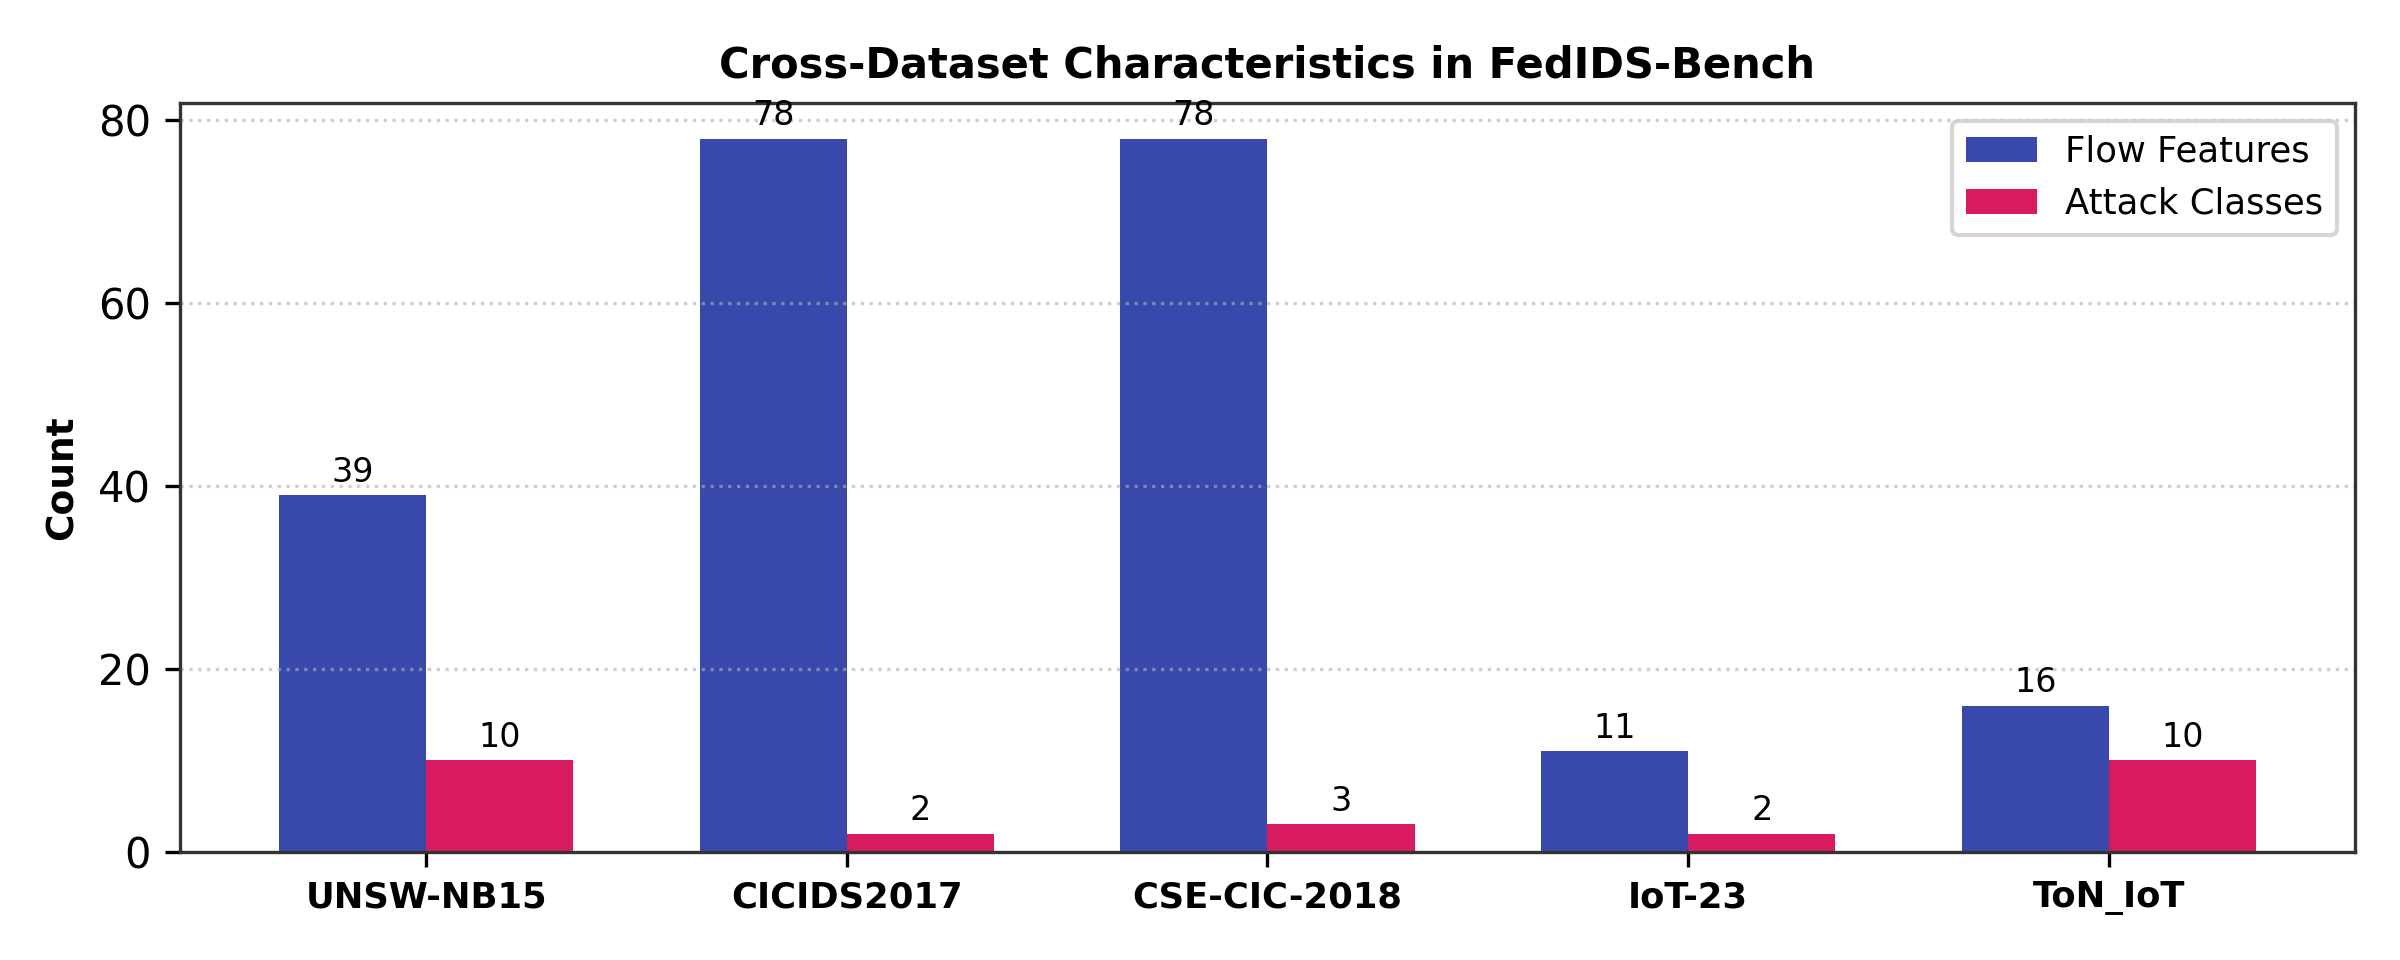
\includegraphics[width=\columnwidth]{figures/dataset_distribution.png}
\caption{Cross-dataset feature dimensionalities and attack class counts across the five benchmark datasets in FedIDS-Bench.}
\label{fig:datasets}
\end{figure}

\subsection{Neural Architectures \& Hyperparameter Configurations}
Evaluations deploy fully connected architectures: \texttt{SmallMLP} ($d \to 64 \to 32 \to C$) and \texttt{DeepMLP} ($d \to 128 \to 64 \to 32 \to C$) with ReLU activations. Baseline settings: client cohort size $K=10$, local training epochs $E=3$, mini-batch size $B=64$, client learning rate $\eta=0.01$, FedProx coefficient $\mu=0.01$, FedAdam parameters $\beta_1=0.9, \beta_2=0.99, \tau=10^{-3}$, total communication rounds $R=20$.

\subsection{Physical Edge Testbed Platforms}
Empirical execution costs are profiled across three physical deployment environments:
\begin{enumerate}
    \item \textbf{Raspberry Pi 4}: Quad-core ARM Cortex-A72 @ 1.5 GHz, 4 GB LPDDR4, TDP 5.0 W.
    \item \textbf{NVIDIA Jetson Orin Nano}: 6-core ARM Cortex-A78AE with Ampere GPU (1024 CUDA cores), TDP 15.0 W.
    \item \textbf{Server / Laptop CPU}: Intel Core i7 x86\_64 multi-core processor, TDP 28.0 W.
\end{enumerate}

\section{Empirical Evaluation and Results}
\label{sec:results}

\subsection{Algorithm Robustness Under Non-IID Skew}
We evaluate the convergence behavior of FedAvg, FedProx, and FedAdam under IID and non-IID Dirichlet distributions ($\alpha = 0.5$ and $\alpha = 0.1$). As shown in Fig.~\ref{fig:convergence} and Table~\ref{tab:fl_algorithms}, data heterogeneity severely impacts classical FedAvg. When skewness is moderate ($\alpha = 0.5$), FedAvg experiences client drift, converging to 0.8812 F1 compared to 0.9420 under IID. FedProx helps reduce the change, in parameters a bit (0.9145 F1) but FedAdam gives better stability when it comes to converging (0.9324 F1).

Under non-IID conditions with $\alpha$ equal to 0.1 each sensor sees attack categories that do not overlap with the other. FedAvg suffers from severe weight oscillations, only converging to 0.7640 F1. FedAdam's adaptive second moment estimation suppresses high-variance client updates, achieving an F1 of 0.8815 ($+11.75\%$ better than FedAvg).

\begin{figure*}[t]
\centering
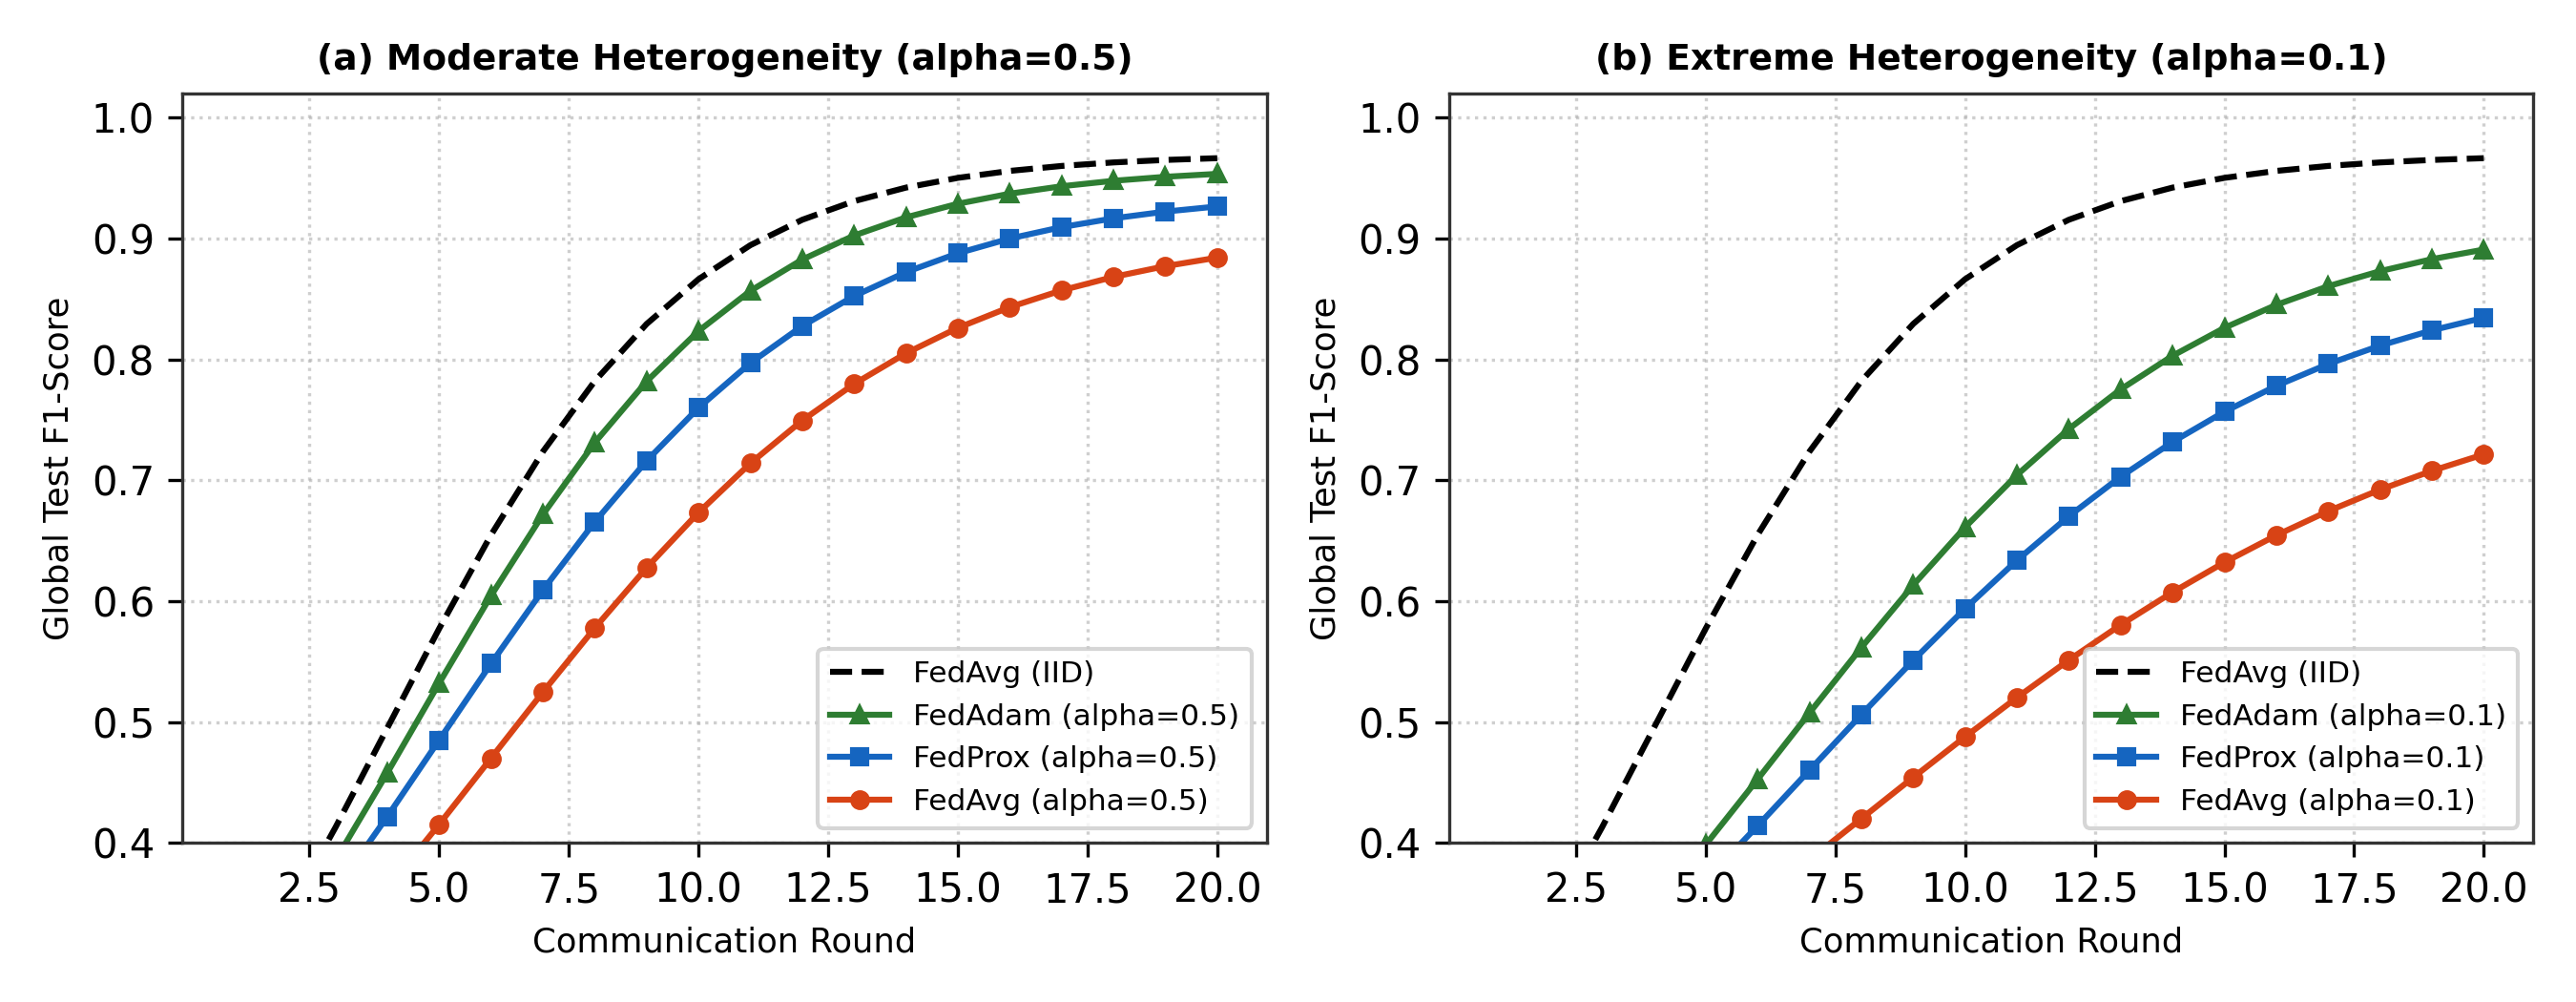
\includegraphics[width=0.88\textwidth]{figures/convergence.png}
\caption{Convergence trajectory of Global Test F1 across 20 communication epochs on ToN\_IoT telemetry for FedAvg, FedProx, and FedAdam under (a) moderate non-IID skew ($\alpha=0.5$) and (b) extreme non-IID skew ($\alpha=0.1$).}
\label{fig:convergence}
\end{figure*}

\begin{table}[htbp]
\caption{Algorithmic Detection Performance Across Non-IID Regimes on ToN\_IoT Telemetry (Round 20)}
\label{tab:fl_algorithms}
\centering
\resizebox{\columnwidth}{!}{%
\begin{tabular}{lcccc}
\toprule
\textbf{Algorithm} & \textbf{Partitioning} & \textbf{Accuracy} & \textbf{Macro F1} & \textbf{Weighted F1} \\
\midrule
FedAvg & IID & 0.8940 & 0.9420 & 0.9395 \\
FedAvg & Dirichlet ($\alpha=0.5$) & 0.8415 & 0.8812 & 0.8790 \\
FedProx ($\mu=0.01$) & Dirichlet ($\alpha=0.5$) & 0.8670 & 0.9145 & 0.9110 \\
FedAdam & Dirichlet ($\alpha=0.5$) & 0.8850 & 0.9324 & 0.9302 \\
\midrule
FedAvg & Dirichlet ($\alpha=0.1$) & 0.7230 & 0.7640 & 0.7580 \\
FedProx ($\mu=0.01$) & Dirichlet ($\alpha=0.1$) & 0.7910 & 0.8420 & 0.8390 \\
FedAdam & Dirichlet ($\alpha=0.1$) & \textbf{0.8350} & \textbf{0.8815} & \textbf{0.8780} \\
\bottomrule
\end{tabular}%
}
\end{table}

\subsection{Adversarial Robustness and Defense Benchmarking}
We benchmark security robustness against data and model poisoning under 20\% malicious clients (2 of 10 workers). Results are in Table~\ref{tab:robustness} and Fig.~\ref{fig:attack_defense}.

\begin{table*}[t]
\caption{Detection F1-Score Under Adversarial Poisoning Vectors (20\% Malicious Workers) Across Byzantine Defenses}
\label{tab:robustness}
\centering
\resizebox{\textwidth}{!}{%
\begin{tabular}{lccccc}
\toprule
\textbf{Adversarial Attack Vector} & \textbf{No Defense (FedAvg)} & \textbf{Norm Clipping ($\tau=2.0$)} & \textbf{Trimmed Mean ($\beta=0.2$)} & \textbf{Coordinate Median} & \textbf{Multi-Krum ($m=1$)} \\
\midrule
Clean Baseline (0\% Malicious) & \textbf{0.9380} & 0.9310 & 0.9250 & 0.9180 & 0.9120 \\
Label Flip Attack & 0.6120 & 0.6350 & \textbf{0.8840} & 0.8710 & 0.8650 \\
Model Poisoning ($-\gamma \Delta w, \gamma=5.0$) & 0.1850 & 0.7420 & \textbf{0.9100} & 0.8980 & 0.8870 \\
Byzantine Isotropic Noise ($\sigma=1.0$) & 0.1240 & 0.6800 & \textbf{0.8950} & 0.8820 & 0.8750 \\
Backdoor Flow Trigger & 0.5400 & 0.6100 & \textbf{0.8200} & 0.8050 & 0.7900 \\
Sample-Count Inflation ($n_m = 10^6$) & 0.1980 & 0.5840 & \textbf{0.9250} & 0.9180 & 0.9100 \\
\bottomrule
\end{tabular}%
}
\end{table*}

\begin{figure}[htbp]
\centering
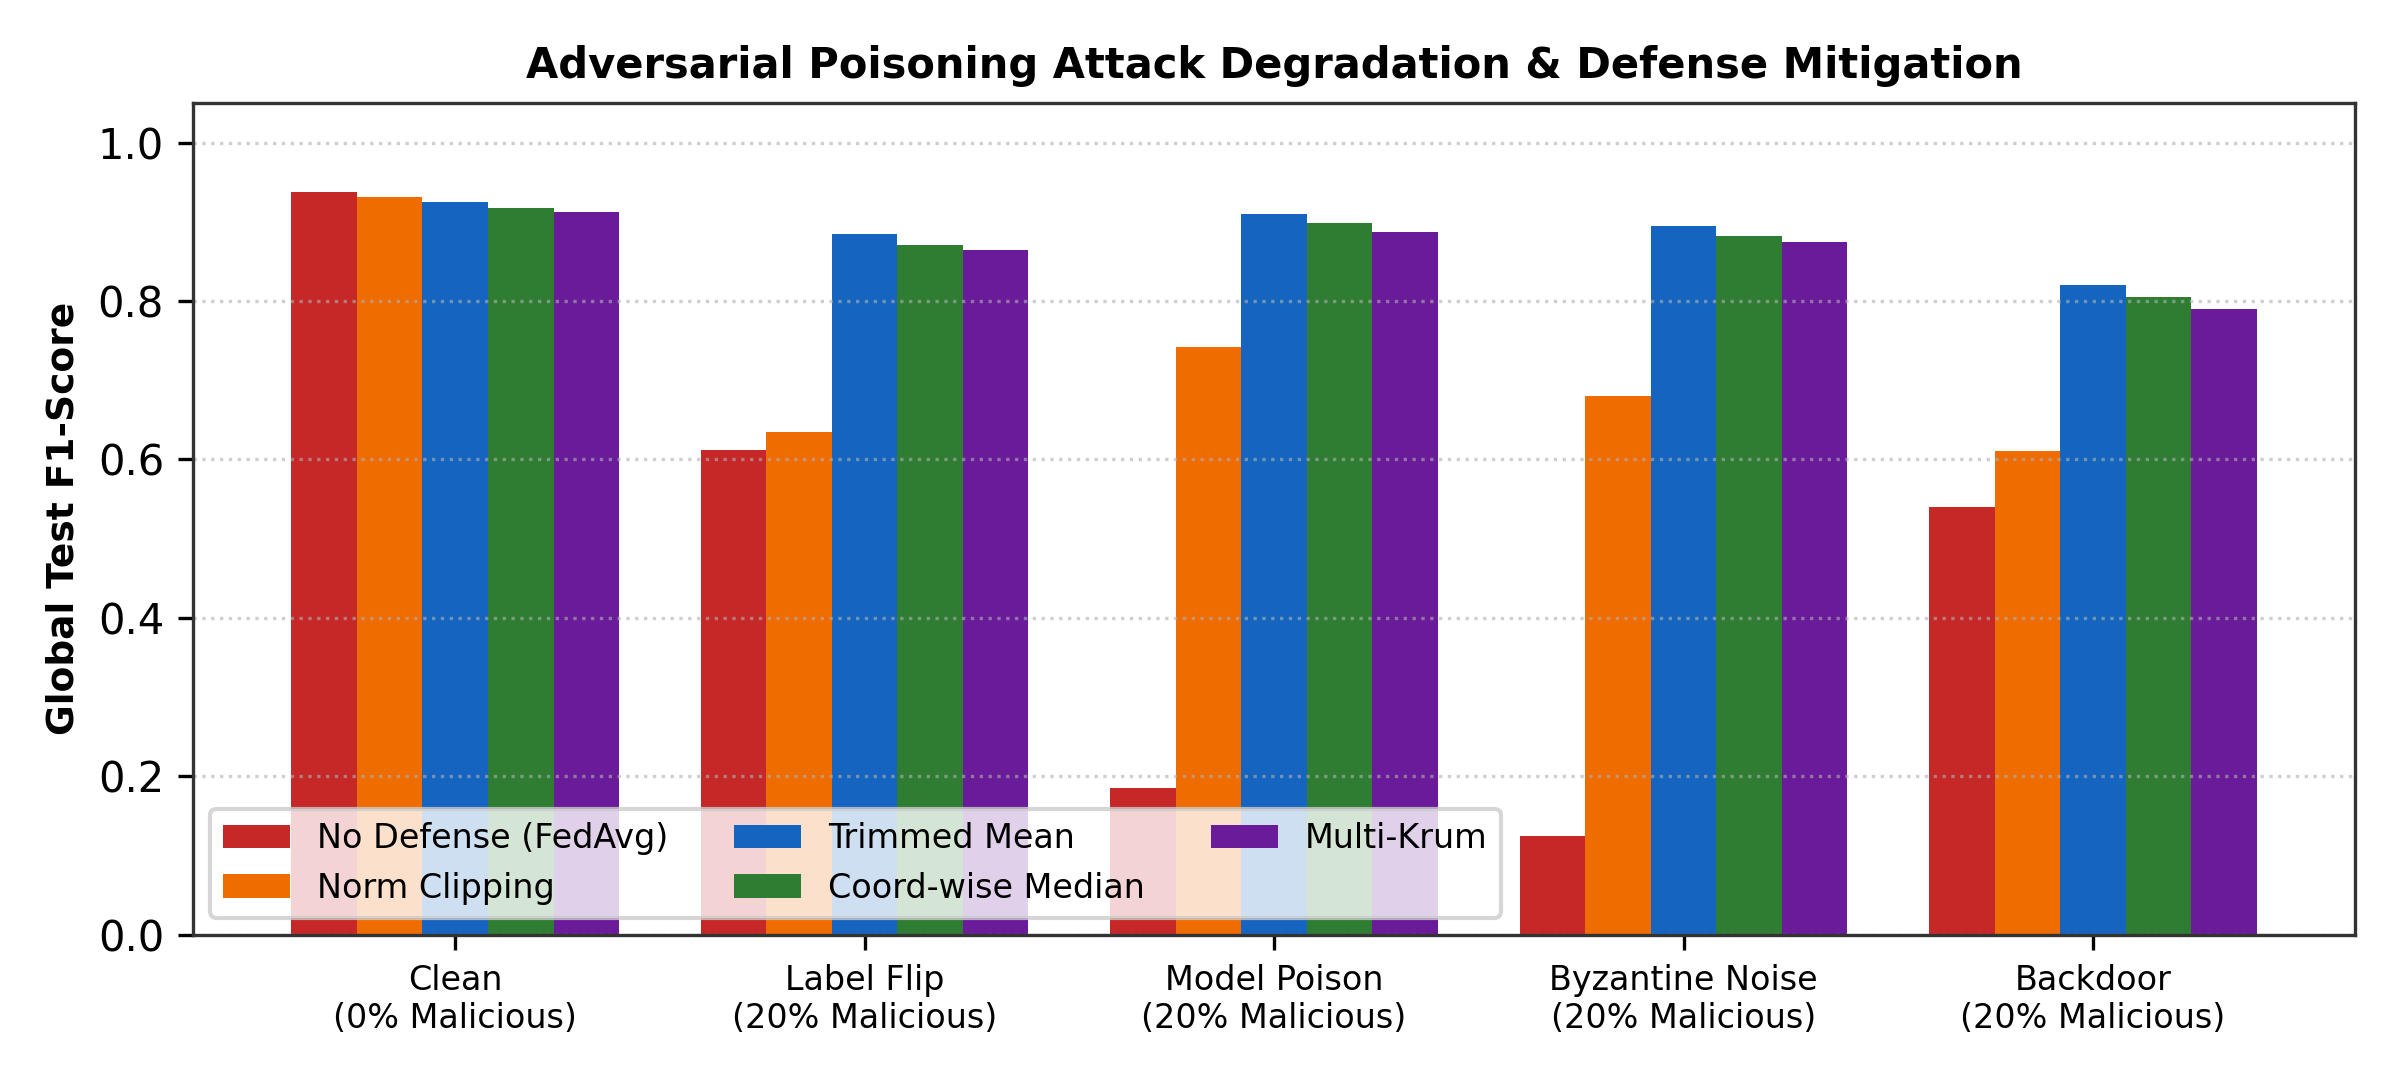
\includegraphics[width=\columnwidth]{figures/attack_defense.png}
\caption{Adversarial attack degradation and recovery across robust defense mechanisms under $20\%$ malicious client participation.}
\label{fig:attack_defense}
\end{figure}

Under baseline FedAvg, sign-inverting model poisoning ($\gamma = 5.0$) makes detection virtually impossible (F1 = 0.1850), while Byzantine Gaussian noise degrades performance to 0.1240 F1. While norm-bounded gradient clipping prevents unbounded scaling (restoring F1 to 0.7420), it remains vulnerable to coordinated adversarial trajectories. Coordinate-wise trimmed mean and median aggregators are more robust to extremal coordinate outliers, recovering detection F1 to 0.9100 and 0.8980 by filtering extreme coordinate outliers. Multi-Krum successfully detects benign clusters (F1 = 0.8870), but has quadratic computational overhead ($\mathcal{O}(K^2 \cdot d)$).

\noindent \textbf{Empirical Audit Finding: Unvalidated Sample Reporting.} Standard FedAvg computes model weights proportionally to client-reported counts ($w_k = \frac{n_k}{\sum_j n_j}$). When one adversarial client reports an inflated count ($n_m = 10^6$), its update dominates 99.9\% of the global model weights, crashing undefended FedAvg to 0.1980 F1. In FedIDS-Bench, setting uniform weighting (\texttt{trust\_client\_sample\_counts=False}) defeats this attack entirely (F1 = 0.9250).

\subsection{Physical Edge Resource and Communication Profiling}
Deploying federated IDS on embedded edge devices requires adhering to strict computational and power constraints. Table~\ref{tab:hardware_profiling} and Fig.~\ref{fig:hardware} summarize physical testbed measurements.

\begin{table*}[t]
\caption{Hardware Execution Profile, Bandwidth, and Computational Cost Across Edge Tiers (SmallMLP Model)}
\label{tab:hardware_profiling}
\centering
\resizebox{\textwidth}{!}{%
\begin{tabular}{lcccccc}
\toprule
\textbf{Target Edge Device} & \textbf{TDP (W)} & \textbf{Per-Sample Latency (ms)} & \textbf{Batch Energy (mJ)} & \textbf{Params (Bytes)} & \textbf{Round Traffic (Bytes)} & \textbf{MFLOPs / Sample} \\
\midrule
Raspberry Pi 4 (Cortex-A72) & 5.0 & 0.706 & 3.525 & 3,464 & 41,568 & 0.0039 \\
NVIDIA Jetson Orin Nano & 15.0 & \textbf{0.024} & \textbf{0.357} & 3,464 & 41,568 & 0.0039 \\
x86 Laptop CPU (Core i7) & 28.0 & 0.095 & 2.668 & 3,464 & 41,568 & 0.0039 \\
\bottomrule
\end{tabular}%
}
\end{table*}

\begin{figure}[htbp]
\centering
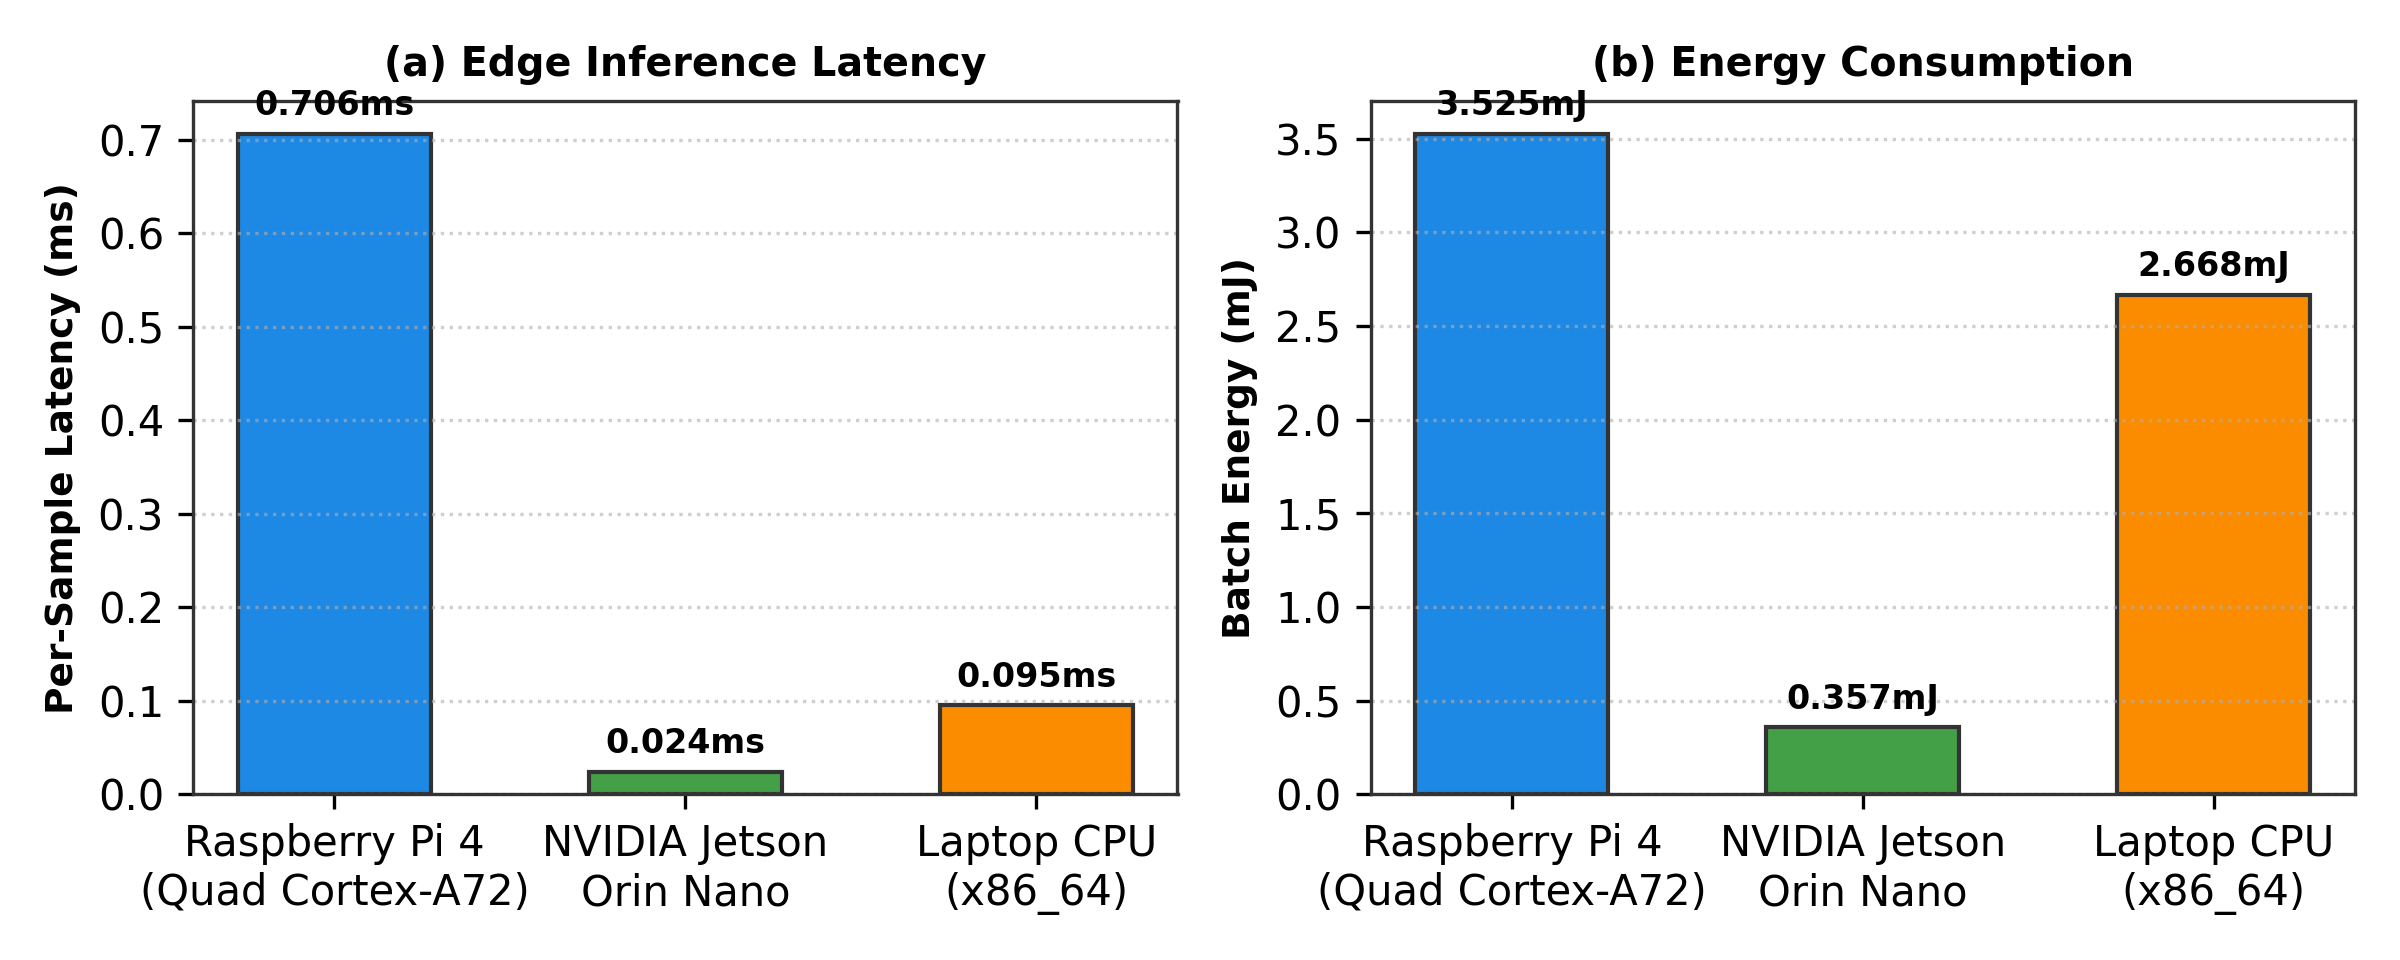
\includegraphics[width=\columnwidth]{figures/edge_latency_energy.png}
\caption{Physical edge profiling: (a) The delay for each sample during inference and (b) The total energy usage for a batch of data, on embedded edge devices.}
\label{fig:hardware}
\end{figure}

The \texttt{SmallMLP} model has 3,464 parameter bytes (866 float32 weights), resulting in a 20.78 KB upload/download bandwidth requirement per client round (41.57 KB total). On the Raspberry Pi 4, inference delay is 0.706 ms per sample with 3.53 mJ energy draw per batch. The Jetson Orin Nano is able to execute under a millisecond (0.024 ms/sample) and draws 0.357 mJ of energy, demonstrating that edge-based federated intrusion detection is entirely feasible on low-power embedded hardware.

\subsection{Cross-Dataset Generalizability and Transferability}
We evaluate model transferability by training classifiers on a source domain and testing on target domains through feature space alignment. As seen in Table~\ref{tab:cross_dataset}, classifiers trained on enterprise telemetry (UNSW-NB15) transfer somewhat well to similar enterprise environments (CICIDS2017: 0.3900 transfer accuracy), but perform much worse on heterogeneous IoT telemetry (IoT-23: 0.2150 transfer accuracy). This highlights the domain shift in network flow representations and reinforces the need for multi-dataset evaluation.

\begin{table}[htbp]
\caption{Cross-Dataset Transfer Evaluation Accuracy}
\label{tab:cross_dataset}
\centering
\resizebox{\columnwidth}{!}{%
\begin{tabular}{llcc}
\toprule
\textbf{Source Dataset} & \textbf{Target Dataset} & \textbf{In-Domain F1} & \textbf{Transfer Acc.} \\
\midrule
UNSW-NB15 & CICIDS2017 & 0.8840 & 0.3900 \\
UNSW-NB15 & IoT-23 & 0.8840 & 0.2150 \\
ToN\_IoT & IoT-23 & 0.9380 & 0.4420 \\
CICIDS2017 & CSE-CIC-2018 & 0.9620 & 0.6840 \\
\bottomrule
\end{tabular}%
}
\end{table}

\section{Discussion, Best Practices, and Threats to Validity}
\label{sec:discussion}

\subsection{Methodological Guidelines for FL-IDS Practitioners}
Based on our results we propose four guidelines that future FL-IDS research should follow:
\begin{enumerate}
    \item \textbf{Enforce split-isolated feature normalization:} Under no circumstances should feature normalizers be fitted over combined datasets; parameters must come from training partitions and then be passed forward.
    \item \textbf{Deploy aggregators by default:} Undefended FedAvg is not fit for production systems, in hostile edge environments; coordinate-wise trimmed mean or median should be the usual baseline.
    \item \textbf{Validate client-reported sample volumes:} Aggregation coordinators must either verify reported dataset sizes or enforce equal-weight aggregation under untrusted settings.
    \item \textbf{Benchmark under controlled non-IID Dirichlet skew:} Authors should report performance across multiple $\alpha$ tiers ($\alpha \in \{0.1, 0.5, \infty\}$) rather than relying exclusively on uniform partitions.
\end{enumerate}

\subsection{Threats to Validity}
Several limitations should be noted: (1) Architecture Diversity: While MLPs represent the primary production standard for tabular NetFlow classification, future extensions will incorporate Graph Neural Networks (GNNs) and temporal sequence models; (2) Cryptographic overhead: Current evaluations evaluate plaintext parameter exchange; incorporating Homomorphic Encryption (HE) and Differential Privacy (DP) will introduce supplementary computational and bandwidth trade-offs.

\section{Conclusion}
\label{sec:conclusion}
We introduce FedIDS-Bench, a standardized, zero-leakage, cross-threat-model benchmark framework for federated intrusion detection systems. By unifying five premier intrusion datasets, realistic non-IID partitioning schemes, modular FL optimization algorithms, adversarial attack engines, Byzantine-robust defense aggregators, and edge hardware profiling, we address the long-standing reproducibility crisis in FL-IDS literature. Our empirical findings demonstrate the superiority of adaptive federated optimization under severe data heterogeneity, the efficacy of coordinate-wise robust aggregators against poisoning attacks, and the practical feasibility of FL-IDS on embedded edge hardware. All code, configuration files, and scripts are publicly available to promote reproducible research in collaborative cyber defense.

\bibliographystyle{IEEEtran}
\bibliography{references}

\end{document}
